% Executive summary of the PGC Editor warm pipeline — two pages,
% one column, for product stakeholders and the senior architect.
% Full technical treatment: pgc-warm-pipeline.tex (same directory).
\documentclass[10pt]{article}
\usepackage[a4paper, margin=23mm, bottom=26mm]{geometry}
\usepackage{microtype}
\usepackage{booktabs}
\usepackage{tikz}
\usetikzlibrary{arrows.meta, positioning, shapes.geometric, fit}
\usepackage{enumitem}
\usepackage[hidelinks]{hyperref}
\usepackage{titlesec}
\titleformat{\section}{\normalfont\large\bfseries}{\thesection}{0.8em}{}
\titlespacing{\section}{0pt}{14pt}{5pt}
\setlist{nosep, leftmargin=1.4em}
\setlength{\parskip}{4pt}\setlength{\parindent}{0pt}
\def\LuaTeX{Lua\TeX}
\def\LuaLaTeX{Lua\LaTeX}
\def\cs#1{\texttt{\char`\\#1}}

\begin{document}

{\LARGE\bfseries The PGC Editor warm pipeline}\\[2pt]
{\large Executive summary for architecture review}\\[4pt]
{\small Srikanth Mohankumar · TNQ Tech · July 2026 ·
full article: \texttt{pgc-warm-pipeline.pdf}}

\vspace{2pt}\hrule\vspace{6pt}

\section*{What changed}

Every correction in the PGC Editor used to pay a full, stateless
XML$\,\to\,$\TeX$\,\to\,$PDF pipeline: 18--25\,s per build, of which
about 72\% was the \TeX{} template preamble --- work that never depends
on the edit. The warm pipeline keeps that work \emph{resident in
processes} instead of redoing it:

\begin{center}
\small
\begin{tabular}{@{}lccl@{}}
\toprule
Operator action & before & after & how\\
\midrule
Build a correction & 18--25\,s & \textbf{3--5\,s} &
  preamble-resident \LuaTeX{} engine, warm converter\\
Check a keystroke & a full build & \textbf{$\sim$0.2\,s} &
  one paragraph re-typeset, drawn live over the PDF\\
Output fidelity & --- & identical &
  golden-gated: equivalent \texttt{.tex}, identical PDF text\\
\bottomrule
\end{tabular}
\end{center}

Measured on production articles: ACS 18.8\,s$\to$4.7\,s (4.0$\times$),
Sage 22.5\,s$\to$3.1\,s (7.3$\times$), operator-observed in the live
editor 22.7\,s$\to$4.1\,s. Paragraph previews: 164\,ms median,
line-break-identical to the full build to the scaled point.

\section*{How it works, in one paragraph each}

\textbf{Warm build engines.} A Lua harness turns \texttt{lualatex} into
a server: it typesets the article's preamble once, then waits on a pipe.
A build sends only the document body; the engine typesets it exactly as
a normal run would and exits cleanly, producing a valid PDF. Engines are
deliberately \emph{single-shot} --- production templates leak float and
tagging state across body re-runs (verified: a second run silently lost
figure pages) --- so every build gets first-run semantics by
construction, and a replacement engine prewarms in the background while
the operator reads the result.

\textbf{Keystroke previews.} During each warm build the engine also
records, per paragraph, its full typesetting context ($\sim$25
line-breaking parameters, the active font, page position). A separate
per-article \emph{serve} engine can then re-typeset any single
paragraph inside an unshipped box in $\sim$10--100\,ms --- safe to
reuse thousands of times because no page-building machinery ever runs
--- and the browser draws the returned glyphs over the stale PDF at
engine-exact positions while the operator types. The next real build
replaces the overlay with truth.

\begin{center}
\resizebox{0.98\textwidth}{!}{% Figure 1 — PGC Editor warm-pipeline architecture (wide, two-column span)
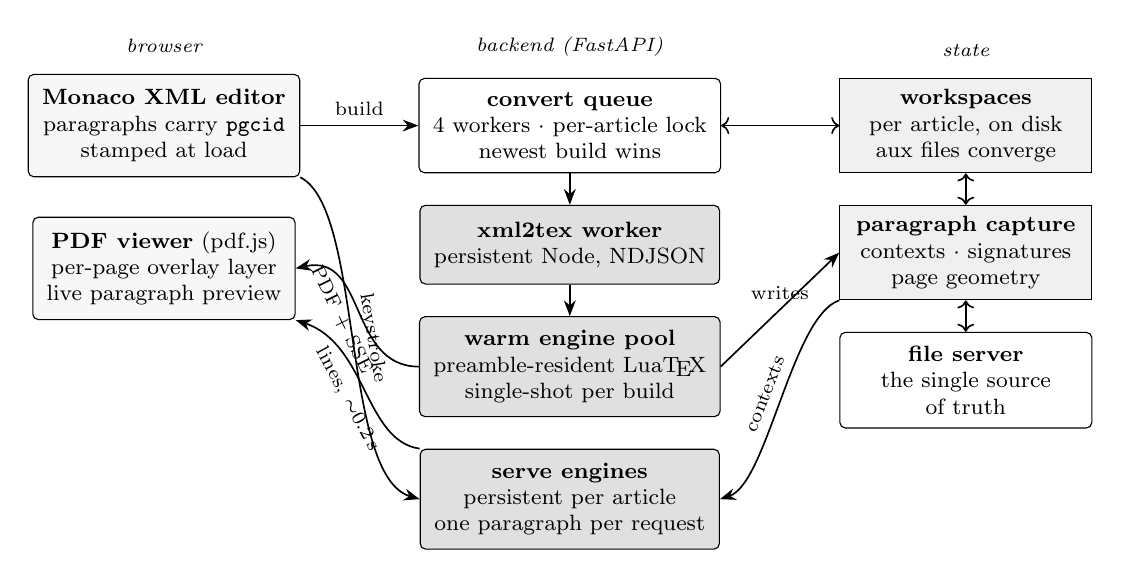
\begin{tikzpicture}[
  font=\footnotesize,
  box/.style={draw, rounded corners=2pt, align=center, inner sep=5pt,
              minimum height=8mm},
  store/.style={draw, align=center, inner sep=4pt, fill=black!6},
  eng/.style={box, fill=black!12},
  arr/.style={-{Stealth[length=2mm]}, semithick},
  node distance=6mm and 10mm]

  % browser column
  \node[box, fill=black!3, minimum width=32mm, minimum height=13mm]
    (editor) {\textbf{Monaco XML editor}\\ paragraphs carry \texttt{pgcid}\\ stamped at load};
  \node[box, fill=black!3, minimum width=32mm, minimum height=13mm, below=5mm of editor]
    (viewer) {\textbf{PDF viewer} (pdf.js)\\ per-page overlay layer\\ live paragraph preview};
  \node[font=\scriptsize\itshape, above=1.5mm of editor] {browser};

  % backend column
  \node[box, right=15mm of editor, minimum width=38mm, minimum height=11mm]
    (queue) {\textbf{convert queue}\\ 4 workers $\cdot$ per-article lock\\ newest build wins};
  \node[eng, below=4mm of queue, minimum width=38mm, minimum height=10mm]
    (x2t) {\textbf{xml2tex worker}\\ persistent Node, NDJSON};
  \node[eng, below=4mm of x2t, minimum width=38mm, minimum height=11mm]
    (pool) {\textbf{warm engine pool}\\ preamble-resident \LuaTeX\\ single-shot per build};
  \node[eng, below=4mm of pool, minimum width=38mm, minimum height=11mm]
    (serve) {\textbf{serve engines}\\ persistent per article\\ one paragraph per request};
  \node[font=\scriptsize\itshape, above=1.5mm of queue] {backend (FastAPI)};

  % state column
  \node[store, right=15mm of queue, minimum width=32mm, minimum height=10mm]
    (ws) {\textbf{workspaces}\\ per article, on disk\\ aux files converge};
  \node[store, below=4mm of ws, minimum width=32mm, minimum height=10mm]
    (cap) {\textbf{paragraph capture}\\ contexts $\cdot$ signatures\\ page geometry};
  \node[box, below=4mm of cap, minimum width=32mm, minimum height=10mm]
    (fs) {\textbf{file server}\\ the single source\\ of truth};
  \node[font=\scriptsize\itshape, above=1.5mm of ws] {state};

  % flows
  \draw[arr] (editor.east) -- node[above, font=\scriptsize]{build} (queue.west);
  \draw[arr] (editor.south east) .. controls +(8mm,-4mm) and +(-10mm,3mm) ..
    node[sloped, above, font=\scriptsize]{keystroke} (serve.west);
  \draw[arr] (queue) -- (x2t);
  \draw[arr] (x2t) -- (pool);
  \draw[arr] (pool.west) .. controls +(-9mm,0mm) and +(9mm,2mm) ..
    node[sloped, below, font=\scriptsize]{PDF + SSE} (viewer.east);
  \draw[arr] (serve.north west) .. controls +(-7mm,1mm) and +(9mm,-3mm) ..
    node[sloped, below, font=\scriptsize]{lines, $\sim$0.2\,s} (viewer.south east);
  \draw[arr] (pool.east) -- node[above, font=\scriptsize]{writes} (cap.west);
  \draw[arr, <->] (queue.east) -- (ws.west);
  \draw[arr, <->] (ws) -- (cap);
  \draw[arr, <->] (cap) -- (fs);
  \draw[arr] (cap.south west) .. controls +(-6mm,-2mm) and +(6mm,2mm) ..
    node[sloped, above, font=\scriptsize]{contexts} (serve.east);
\end{tikzpicture}
}
\end{center}

\section*{Multi-user behavior and capacity}

All warm state is keyed \textbf{per article, never per user}, so
operators on different articles share nothing warm; four builds run in
parallel (as today), each 3--5\,s. Two operators on the same article
serialize on the existing per-article lock, and only the newest queued
build compiles. Capacity planning is by article: a fully warm heavy
article costs 2--3\,GB, engines are hard-capped (6 build + 4 serve)
with LRU eviction and idle reapers, inside an explicit 12\,GB container
limit. Overflow degrades to a one-time cold build, never an error.
Beyond one host, articles shard cleanly: sticky-route by article id;
the file server stays the single source of truth.

\section*{Why it is safe}

\begin{itemize}
\item \textbf{Cold path never removed} --- any warm miss or failure
  falls back automatically; worst case equals current behavior.
\item \textbf{Warm state is disposable} --- engines, workspaces and
  captures are caches over the file server; a crash or OOM kill costs
  one slower build, never data.
\item \textbf{Output-identical, gated per customer} --- an automated
  cold-vs-warm golden comparison guards the flag
  (\texttt{WARM\_ENGINES}); scope is xml2tex2.0 customers, Elsevier/1.x
  untouched.
\item \textbf{Observable and tested} --- \texttt{/metrics} exports
  warm/cold per-stage histograms with a fallback-rate canary; 33-test
  suite plus a 14-scenario end-to-end battery (parity, hostile input,
  engine-death recovery), all passing.
\item \textbf{Known limits are explicit} --- footnotes, display math,
  list items and float captions skip the preview fast path and take the
  normal 3--5\,s build; preview glyphs render at exact positions in the
  article's own typefaces, loaded on demand.
\end{itemize}

\section*{Status and decision points}

All four phases are implemented and verified on branch
\texttt{feature/warm-pipeline} (backend engine pool, load-time
paragraph identity, capture, preview endpoint, live overlay). Proposed
next steps: (1)~QA rollout with \texttt{WARM\_ENGINES=1} for one
xml2tex2.0 customer, watching the fallback canary; (2)~capacity sign-off
on the 12\,GB envelope per backend; (3)~decision on sharding ---
sticky-by-article routing when we scale past one host.

\end{document}
